\subsection{Structure of the Consumer Client}\label{ssec:consumer_client_structure}
The consumer client is a proof of concept of using the REST API.
The consumer client also helped in the process of discovering errors and missing functionalities.
It is build to showcase the different functionalities and the different types of data the REST API can provide.

When a user first opens the consumer client, a login screen will be presented as can be seen in \cref{fig:ConsumerClientLogin}.
Here a username and password is required to log in, the authorization happens through the REST \ac{API}.
\begin{figure}[h]
    \centering
    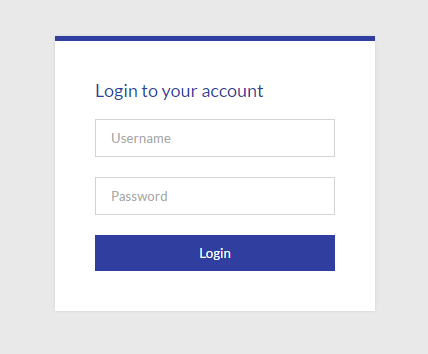
\includegraphics[scale=0.5]{img/ConsumerClientLogin.png}
    \caption{The login page for the consumer client.}
    \label{fig:ConsumerClientLogin}
\end{figure}

When a user is logged in he is firstly presented for an overview of the dashboard.

\begin{figure}[h]
    \centering
    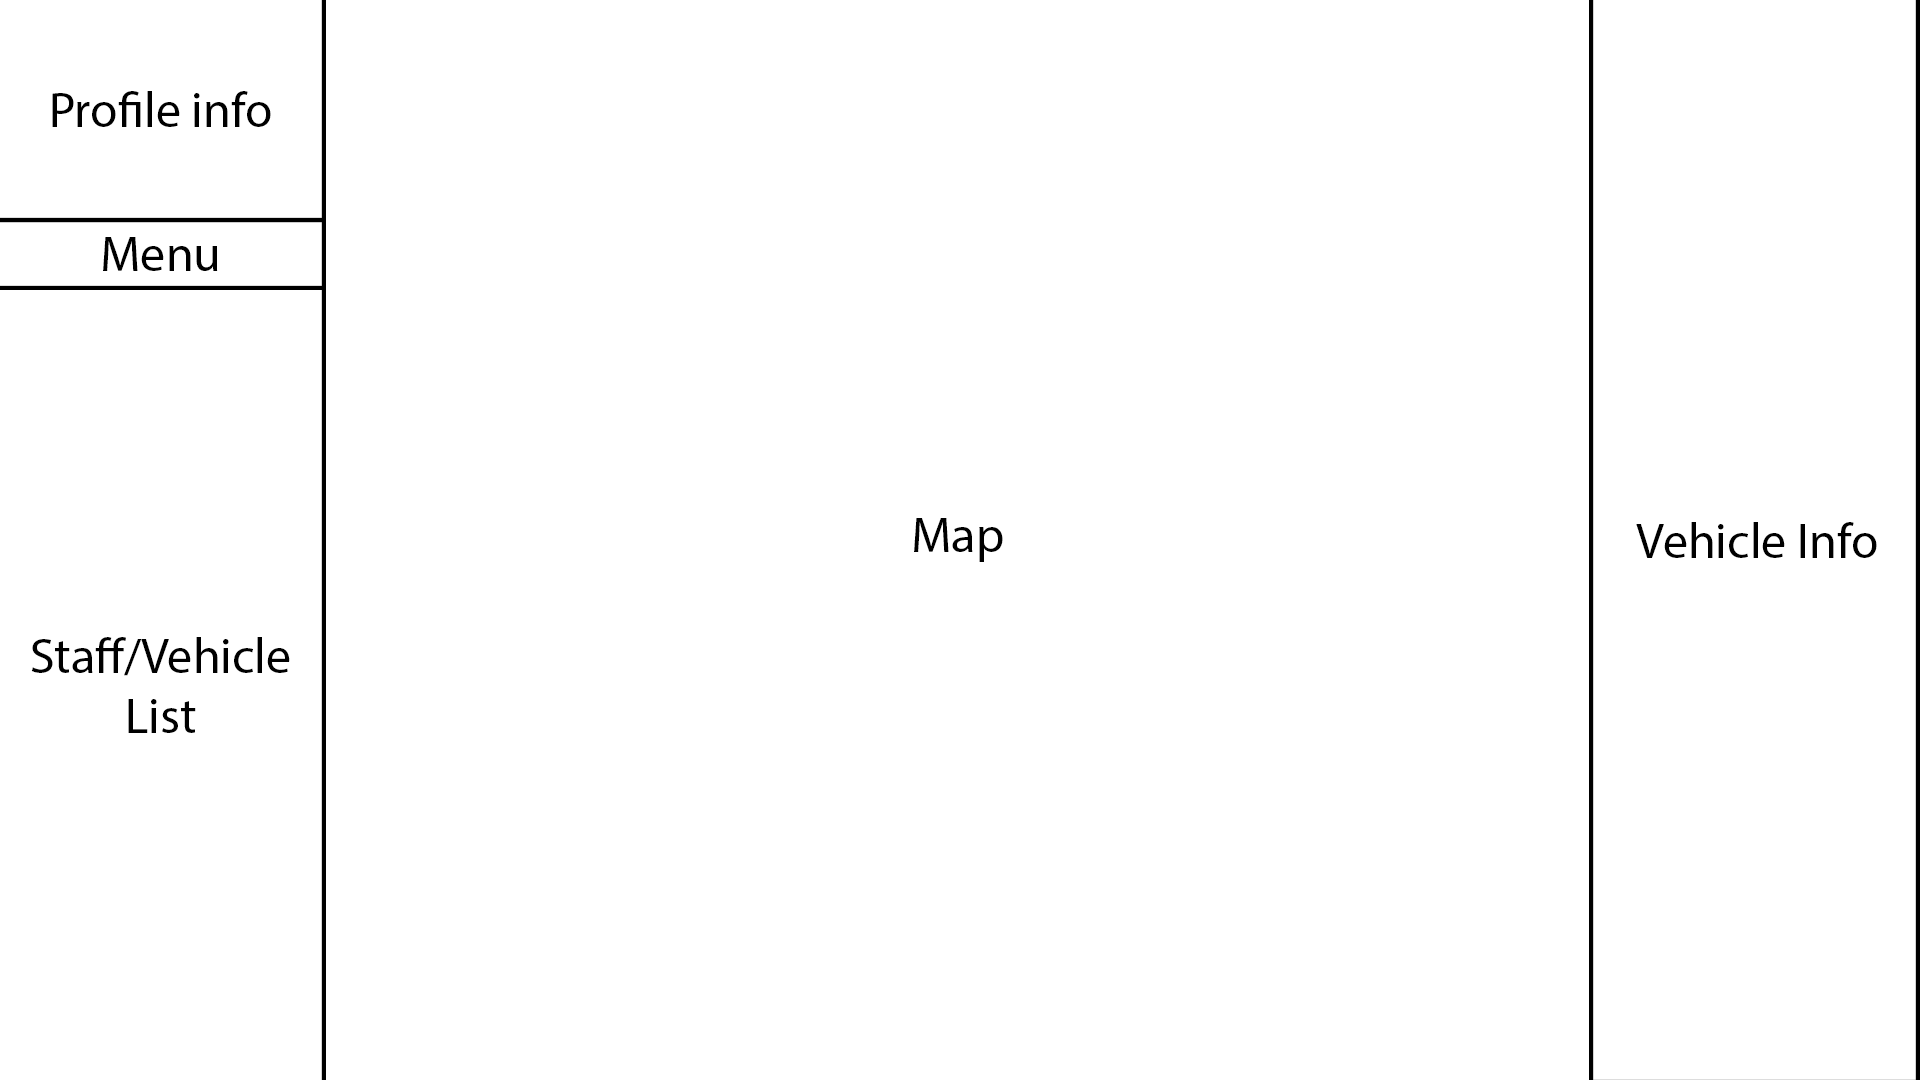
\includegraphics[scale=0.15]{img/ConsumerClientWText.png}
    \caption{A structural overview of the dashboard for the consumer client.}
    \label{fig:ConsumerClientLayout}
\end{figure}

\begin{figure}[h]
    \centering
    \includegraphics[scale=0.35]{img/ConsumerClientExample.png}
    \caption{The consumer client dash board.}
    \label{fig:ConsumerClientExample}
\end{figure}

On \cref{fig:ConsumerClientLayout} the layout of the consumer client can be seen.
The consumer client dash board, which implements the layout from \cref{fig:ConsumerClientLayout}, can be seen on \cref{fig:ConsumerClientExample}.
The user can see his profile information in the top left corner of \cref{fig:ConsumerClientExample}, this information is fetched through the REST API.
More precisely the user's name, username and status is fetched, the stats can either be a user or a super user.
The user's image is also fetched through the REST API, the image is Base64 encoded and represented as a background image, however if the user has no image, a default image will be shown.

Beneath the profile information, a small menu can be seen where the user can choose between employees or vehicles, which toggles between two lists.
If employees are chosen, all employees are shown, where if vehicles are chosen all the vehicles are shown. 
On \cref{fig:ConsumerClientExample} the dash board with vehicles chosen, is shown.

\begin{figure}[h]
    \centering
    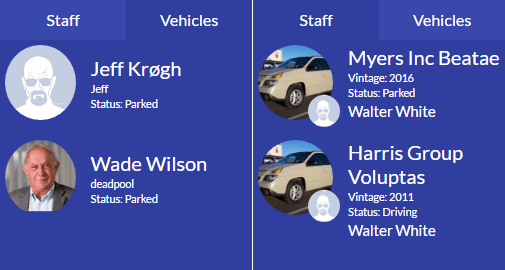
\includegraphics[width=0.3\textwidth]{img/displayOfMenuesInConsumerClient.png}
    \caption{An example of the employee list in the consumer client.}
    \label{fig:ConsumerClientMenus}
\end{figure}

In the list of all the employees, the name, username, image and the current status of the driver can be seen.
An example of the employees list an be seen on \cref{fig:ConsumerClientMenus}.
This status is not like the status shown in the profile information, this status is whether the users are currently driving or parked.
If a user is currently driving, an image of the vehicle will be shown next to the user's image.

In the vehicles list the make and model, an image of the vehicle and whether the vehicle is currently driving or parked can be seen.
If the vehicle is currently driving, a small image of the driver will be shown next to the image of the vehicle.

If the user of the dashboard clicks on either a vehicle or a driver, which is currently driving, the map will automatically be centered around the currently active route the vehicle is driving.

\bigskip
The dashboard also contains an interactive map, which can be seen in the middle of \cref{fig:ConsumerClientExample}.
The user is able to zoom and move around in the map, and through the REST API, the consumer client retrieves the currently active vehicles within the currently visible part of the map.
All the routes which are shown will continually be updated, and movement can be shown in real--time.
All vehicles on the map will by default be represented by a small yellow truck, as seen on \cref{fig:ConsumerClientExample}, however if the vehicle has a custom image, the image will be loaded and shown instead.

All the routes which are drawn on the map are polypaths. 
These paths are drawn between the different GPS coordinates which the producer client sends to the REST API.
A polypath is a line drawn on the interactive map, between an ordered list of GPS coordinates.
Since it is the producer client, which sends the position data from the vehicle and it is this data which the consumer client displays,
a producer client is required.

When a vehicle is clicked, a menu in the right side will be shown, this menu currently contains nothing, but could be used to show more advanced vehicle information, for instance live vehicle data, and previous routes the vehicle has driven.

\bigskip
The consumer client allows for a fast overview of the entire fleet, while also granting the company an opportunity to track its vehicles in real--time on the map and show the current information at the same time.

Since the company is able to track the vehicles in real--time, the consumer client could be used to help prevent future damages to the vehicles.
This can be done by analysing either the real--time data, or by looking for anomalies or deviations in the data from previous routes.
